\documentclass{article}
% General document formatting
\usepackage[margin=1in]{geometry}
\usepackage[parfill]{parskip}
\usepackage[utf8]{inputenc}

\def\mySfFamily{\fontfamily{cmbr}\selectfont\sffamily}
 
% Related to math
\usepackage{amsmath, amssymb, amsfonts, amsthm}
\allowdisplaybreaks
\usepackage[shortlabels]{enumitem}
\usepackage{verbatim}
\usepackage{xcolor}
\usepackage{subcaption}
\usepackage{mathtools}

%bibliography
\usepackage[natbib,backend=biber]{biblatex}
\addbibresource{bibliography.bib}


\usepackage{listings}
\lstset{ 
    language=Promela, % choose the language of the code
    basicstyle=\fontfamily{pcr}\selectfont\footnotesize\color{black},
    keywordstyle=\color{black}\bfseries, % style for keywords
    numbers=none, % where to put the line-numbers
    numberstyle=\tiny, % the size of the fonts that are used for the line-numbers     
    showspaces=false, % show spaces adding particular underscores
    showstringspaces=false, % underline spaces within strings
    showtabs=false, % show tabs within strings adding particular underscores
    frame=single, % adds a frame around the code
    tabsize=2, % sets default tabsize to 2 spaces
    captionpos=b, % sets the caption-position to bottom
    breaklines=true, % sets automatic line breaking
    breakatwhitespace=false, 
}
\usepackage{graphicx}

% proofs
\newcommand{\pre}{\textbf{Precondition: }}
\newcommand{\hyp}{\textbf{Hypothesis: }}

% LTL formulae
\newcommand{\eventually}{\lozenge} %<>
\newcommand{\always}{\square} %[]
\newcommand{\nextstep}{\bigcirc} %O
\newcommand{\until}{\mathsf{\, U \,}} %U
\newcommand{\weakuntil}{\mathsf{\, W \,}} %W
\newcommand{\true}{\text{true}} %true
\newcommand{\ifff}{\, \text{ iff } \,} %iff
\newcommand{\false}{\, \text{false} \,} %iff


\title{Final Report: Model Checking the SIP Protocol with Spin}
\author{Ying Wang \& Fabian Marquart}


\begin{document}

\maketitle


\section{Introduction}

This project's goal is to gain practical experience with the state-of-the-art model checker SPIN in modeling and verifying concurrent systems. The system to be modeled is the Session Initiation Protocol (SIP), a communication protocol for establishing, maintaining, and terminating multimedia sessions such as those used by Voice over Internet applications. Spin and its input language Promela are used to (1) model certain aspects of the SIP protocol, to (2) specify high level properties that the model should satisfy, and to (3) verify whether the specified properties are indeed satisfied \cite{leue}.

\section{The SIP protocol}

The Session Initiation Protocol (SIP) is a signaling, presence, and instant messaging protocol developed to set up, modify, and tear down multimedia sessions; request and deliver presence; and send and receive instant messages \citep[1]{sip}.

\subsection{A Simple Session Establishment Example}

\begin{figure}[h]
\centering
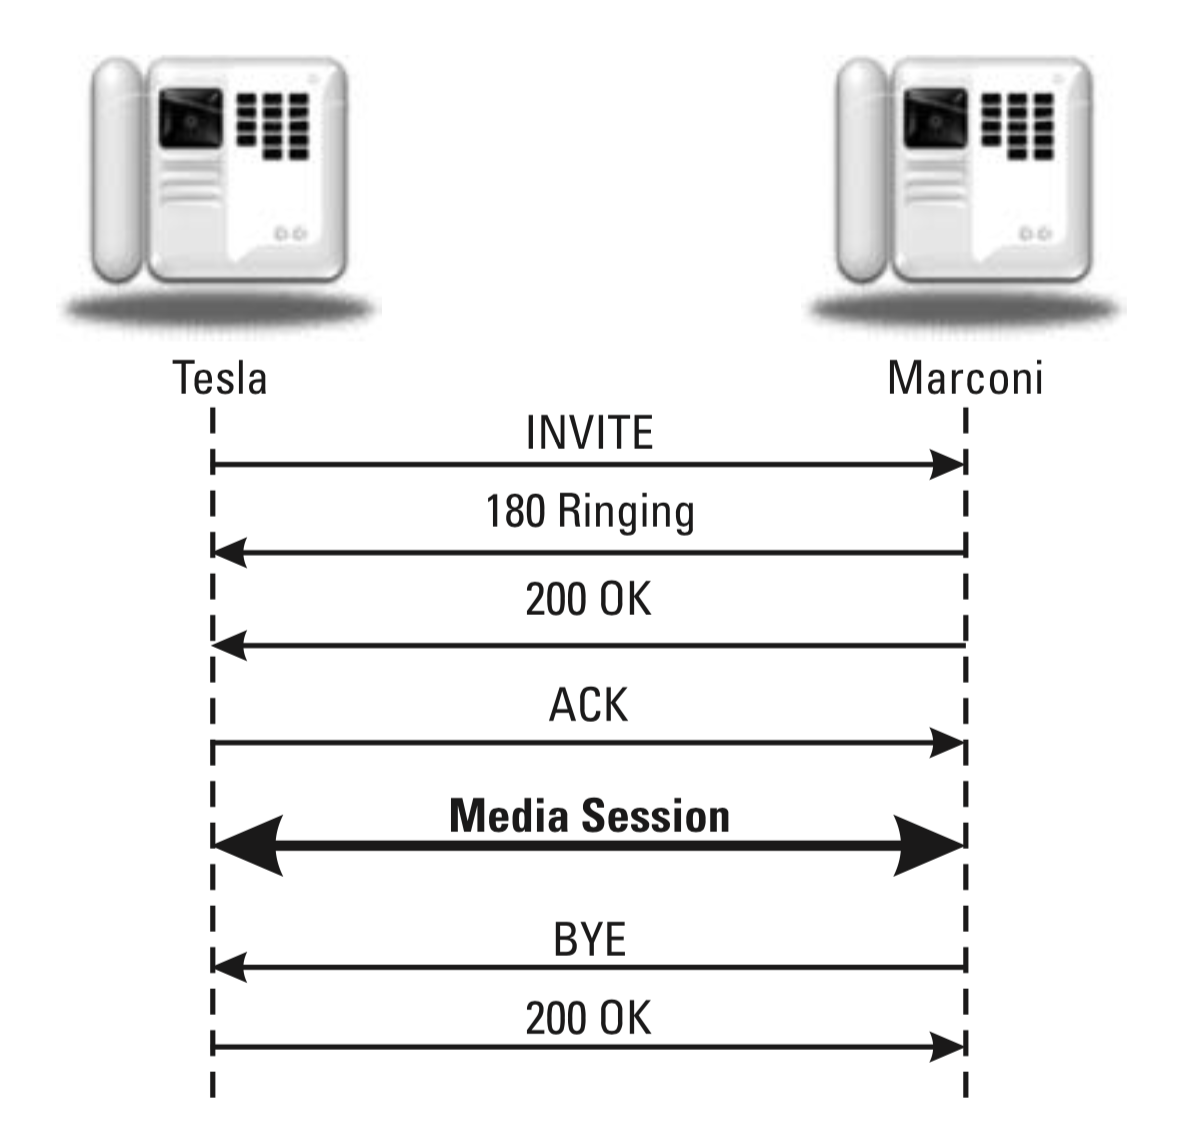
\includegraphics[width=0.4\textwidth]{images/sip_simple.png}
\caption{A simple SIP session establishment example, adapted from \citep[24]{sip}.}
\label{sip_simple}
\end{figure}

Session establishment in SIP starts with an \texttt{invite} message by the client, called Tesla in
Figure \ref{sip_simple}. The server answers with a \texttt{ringing}, sometimes called \texttt{trying} message.
When ready, it sends an \texttt{ok} message to the client. Finally, the client answers with an aknowledgement
message \texttt{ack}, and the multimedia session begins. 

Now, when both agents are finished sending their audio or video data, the server closes the session with
a \texttt{bye} message, which the client answers with another \texttt{ok}.


\subsection{SIP Call with a Proxy Server}

Most of the time, the agents using SIP to call each other do not know each other's IP address, for reasons
such as dynamic reassignment of IP addresses. For this purpose, a proxy server that sits between client
and server forwards the messages between both, as shown in Figure \ref{sip_proxy}.

\begin{figure}[h]
\centering
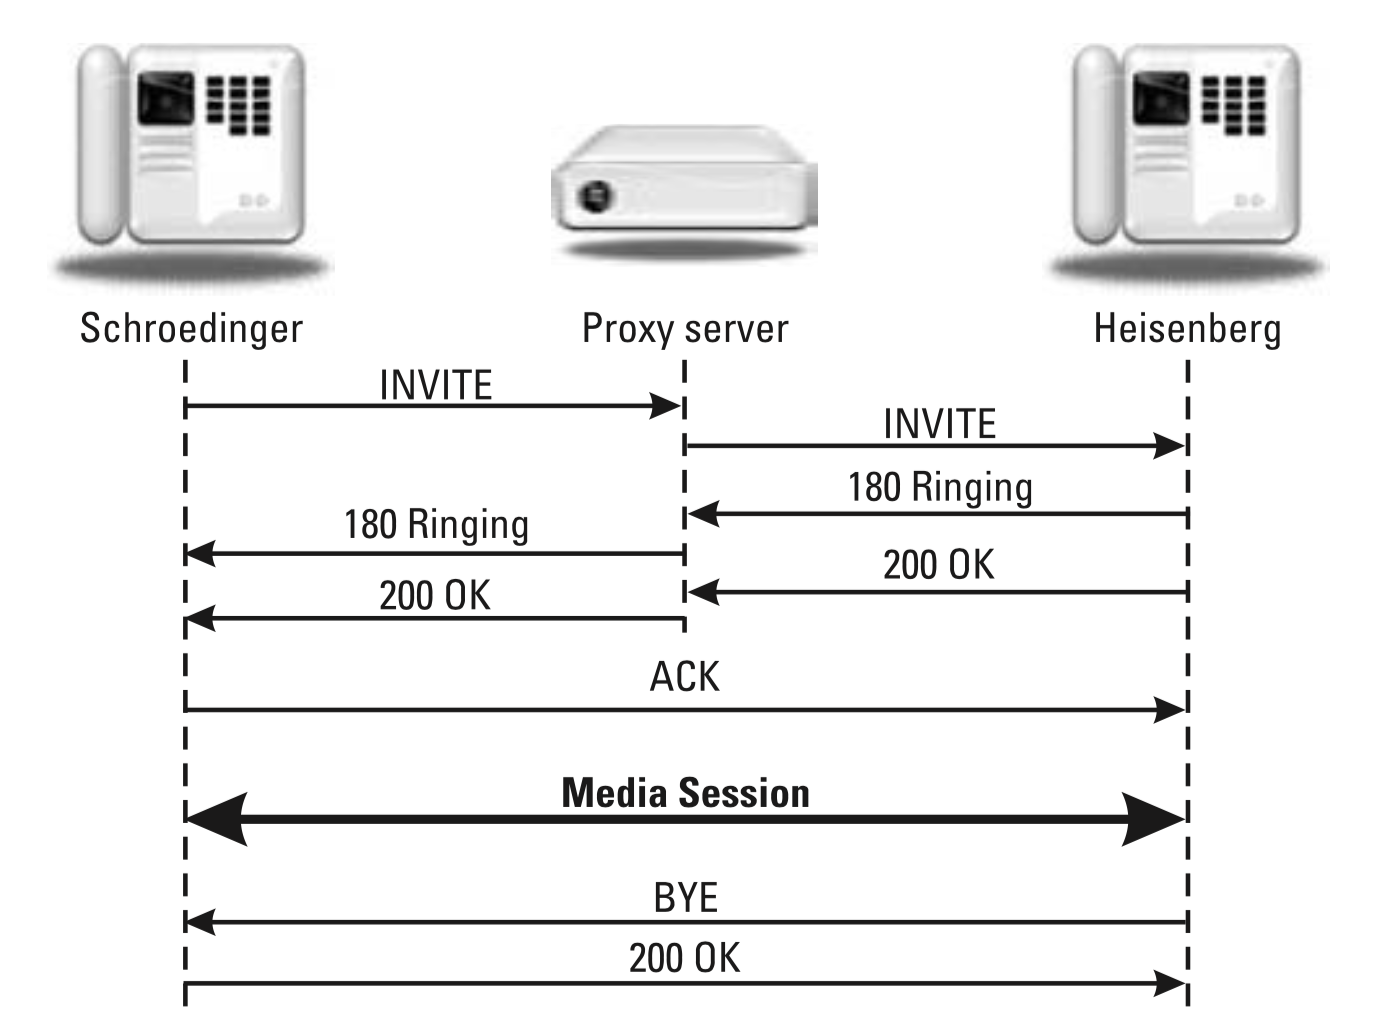
\includegraphics[width=0.57\textwidth]{images/sip_proxy.png}
\caption{SIP call example with a proxy server, adapted from \citep[32]{sip}.}
\label{sip_proxy}
\end{figure}




\section{Model Checking with SPIN and Promela}


\section{Linear Temporal Logic}

\cite{modelchecking}


\section{Requirements}

\subsection{Model}

The model should contain at least two user agents and two proxies. All scenarios related to
setting up and terminating sessions should be modeled. User agents should be able to behave as
client and as server.

\begin{itemize}
\item Client behavior
	\begin{itemize}
	\item sending the requests INVITE, ACK and CANCEL for setting up
		sessions
	\item sending the request BYE for terminating sessions
	\end{itemize}
\item Server behavior
	Sending corresponding responses to requests of client including:
	\begin{itemize}
	\item accepting a request
	\item rejecting a request
	\item server error to fulfill a request
	\end{itemize}
\end{itemize}

The behavior of the transaction user layer must be modeled, including client transactions and server transactions. Any user agent should be able to have multiple sessions at a time. Proxies may be stateless.
The optional aspects of the SIP protocol include (1) registration, (2) dialogs (3) querying,
(4) modifying sessions, (5) stateful proxies, (6) transport layer behavior,
(7) forking and merging requests, among others irrelevant to the above mandatory aspects to be modeled.

\subsection{Properties}

High level properties that the model should satisfy are suggested.
These should include at least two safety properties and two liveness properties.
The model is simulated using Spin to check whether the properties specified are violated.

\subsection{Verification}

The suggested properties are expressed in LTL formulae. Spin is used to model check these properties.
In case a property is violated, the obtained counterexample is analyzed and the cause of the property violation
is identified. 


\section{The Model}

The model consists of two proctypes: an agent and a proxy. The agent has an \texttt{idle} state, where
it can choose between client and server behavior.


\subsection{Implementation}

\subsection{Properties}

\begin{enumerate}
	\item Agents can have two sessions at the same time. One session is initiated by the agent itself, another session is initiated by the other agent.
	
	$ \varphi_1 = \eventually (A.mediaSessionClient \wedge A.mediaSessionServer) $
		
	\item Eventually agent A is able to send another invite to agent B after sending an invite to agent B.
	
	$ \varphi_2 = \always (A.inviting \to \eventually (invitesent_A = 0 \wedge A.idle) \wedge B.inviting
	\to \eventually (invitesent_B = 0 \wedge B.idle))$
	
	\item If the agent cancel its invitation, it is unable to initial a media session corresponding to this invitation.

	$\varphi_3 = \always((\neg cancelsent_A = 1 \wedge A.mediaSessionClient) \wedge \neg(cancelsent_A = 1 \wedge A.mediaSessionClient) )$
	
	
	\item If agent A send an invitation to agent B, it will unable to send another invitation to B until the
	invitation either leads to a media session or it is canceled.
	
	$\varphi_4 = \always(A.inviting \to \eventually(A.inviting \wedge (\neg A.inviting \until A.idle))) \wedge \always(B.inviting \to \eventually(B.inviting \wedge (\neg B.inviting \until B.idle)))$
	
\end{enumerate}


\subsection{Verification}



\section{Conclusion}




\end{document}